\documentclass[a4paper,14pt]{article}
\usepackage{float}
\usepackage{extsizes}
\usepackage{amsmath}
\usepackage{amssymb}
\everymath{\displaystyle}
\usepackage{geometry}
\usepackage{fancyhdr}
\usepackage{multicol}
\usepackage{graphicx}
\usepackage[brazil]{babel}
\usepackage[shortlabels]{enumitem}
\usepackage{cancel}
\columnsep=2cm
\hoffset=0cm
\textwidth=8cm
\setlength{\columnseprule}{.1pt}
\setlength{\columnsep}{2cm}
\renewcommand{\headrulewidth}{0pt}
\geometry{top=1in, bottom=1in, left=0.7in, right=0.5in}

\pagestyle{fancy}
\fancyhf{}
\fancyfoot[C]{\thepage}

\begin{document}
	
	\noindent\textbf{8FMA34, 8FMA35~Matemática} 
	
	\begin{center}Problemas envolvendo conversão de unidades (Versão estudante)
	\end{center}
	
	\noindent\textbf{Nome:} \underline{\hspace{10cm}}
	\noindent\textbf{Data:} \underline{\hspace{4cm}}
	
	%\section*{Questões de Matemática}
	
    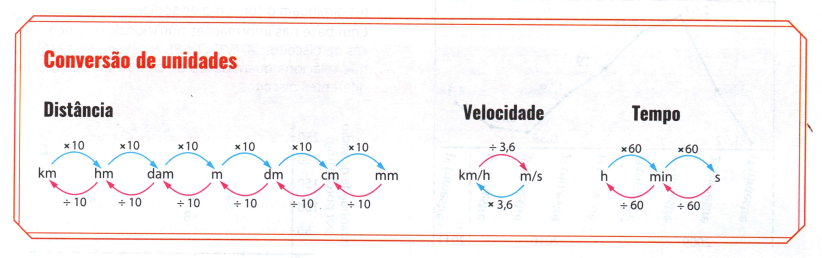
\includegraphics[width=1\linewidth]{8FMA34_imagens/imagem1}
    \begin{multicols}{2}
    	\begin{enumerate}
    		\item A quantos km/h correspondem 20 m/s? \\\\\\\\\\\\
    		\item 36 km/h correspondem a quantos m/s? \\\\\\\\\\\\
    		\item 9 cm/min correspondem a quantos m/s? \\\\\\\\\\\\
    		\item Um ciclista percorre 250 metros a cada 20 segundos. Qual é a sua velocidade em quilômetros por hora? \\\\\\\\\\
    		\item 
    		\begin{enumerate}[a)]
    			\item Um nadador atravessa 12 vezes uma piscina de 25 m em 5 min. Qual é a sua velocidade em km/h? \\\\\\\\\\
    			\item Agora é a sua vez! Monte um exercício como o item anterior e depois resolva-o. \\\\\\\\
    		\end{enumerate}
    	    \item Quando jogava boliche, Renato percebeu que as bolas levavam, em média, 4 segundos para atingir os pinos. Alguém havia dito que isso correspondia a uma velocidade média de 16,2 km/h. Qual é o comprimento da pista de boliche? \\\\\\\\\\\\\\\\\\\\
    	    \item Um ônibus andou 04h25min a uma velocidade média de 65 km/h. Após uma parada de 15 min, reiniciou a viagem, andando 03h40min a 85 km/h.
    	    \begin{enumerate}[a)]
    	    	\item Qual foi o tempo de viagem? \\\\\\\\\\\\\\
    	    	\item Qual foi a distância percorrida pelo ônibus na viagem? \\\\\\\\\\\\
    	    \end{enumerate}
            \item Um motociclista andou metade de um percurso de 420 km à uma velocidade média de 50 km/h e a outra metade à velocidade média de 70 km/h. Quanto tempo levou para fazer a viagem? \\\\\\\\\\\\\\\\\\\\\\\\
            \item Breno pretende visitar sua família numa cidade situada no alto de uma montanha, distante 320 quilômetros da cidade em que mora. O trecho plano da viagem, ele pretende percorrer a uma velocidade média de 80 km/h, o que levará exatamente 3 horas. Se ele percorrer o trecho de subida da montanha a uma velocidade média de 50 km/h, quanto tempo levará a subida? \\\\\\\\\\\\\\\\\\\\
            \item A velocidade de um carro é de 144 km/h. Quantos metros por segundo ele percorre? \\\\\\\\\\\\\\
            \item A milha marítima é representada pelo símbolo mi; tem-se 1 mi = 1852 m. Tradicionalmente, a velocidade de embarcação é expressa em nós. Por definição: \\
            \begin{center}
            	1 nó = 1 $\frac{\text{milha}}{\text{hora}}$ = 1 $\frac{\text{mi}}{\text{h}}$ 
            \end{center}`
            Um torpedeiro desenvolve a velocidade $v = 32$ nós. Essa velocidade equivale aproximadamente a:
            \begin{enumerate}[a)]
            	\item $\frac{1}{150}$~mi/min
            	\item 59 km/h
            	\item $\frac{1}{80}$~mi/s
            	\item 72 km/h
            	\item 23 km/h \\\\\\\\\\\\\\\\\\\\
            \end{enumerate}
            \item A fila na entrada de um show tem aproximadamente 200 m de comprimento, e 300 pessoas se distribuem de maneira uniforme (fila indiana). Ao abrir a porta, as pessoas começam a passar, uma a uma, pelo detector de metais, caminhando durante 2 minutos. Considerando esse período de tempo, qual é o número de pessoas que passaram pelo detector de metais? E qual é o comprimento da fila de pessoas que ainda não passaram? \\\\\\\\\\\\\\\\\\\\
            \item A velocidade de um carro em um trecho de uma estrada é constante e igual a 120 km/h. Caso a velocidade fosse $\frac{3}{5}$ da velocidade inicial, ele gastaria 25 minutos para percorrer esse trecho. Qual foi o tempo gasto indo a 120 km/h? \\\\\\\\\\\\\\
            \item A distância, por estrada de rodagem, entre Pelotas e Teresina é de 4024 km. Um ônibus demora dois dias e duas horas desde a saída de Pelotas até a chegada a Teresina, incluindo paradas para refeições, abastecimentos, etc. A velocidade média desse ônibus, durante os dois dias e duas horas de viagem é, em km/h, igual a:
            \begin{enumerate}[a)]
            	\item 70,82
            	\item 75,70
            	\item 80,48
            	\item 86,18
            	\item 92,43 \\\\\\\\\\\\\\\\\\\\
            \end{enumerate}
            \item Um ônibus faz um percurso de 154 km entre as cidades de São José dos Campos e Campinas, parando em Atibaia para um descanso. Saindo às 9 h de São José dos Campos, o ônibus percorre 90 km até chegar em Atibaia, com uma velocidade constante de 60 km/h neste trecho, permanecendo lá por 20 minutos.
            \begin{enumerate}[a)]
            	\item Qual é a distância entre Atibaia e Campinas? \\\\\\\\\\\\\\\\\\\\
            	\item Quanto tempo o ônibus leva para percorrer o trecho entre São José dos Campos e Atibaia? \\\\\\\\\\\\\\\\\\\\
            	\item Qual é o horário em que o ônibus chegou em Campinas se ele levou 40 minutos para ir de Atibaia até Campinas? \\\\\\\\\\\\\\\\\\\\\\\\\\
            \end{enumerate}
            \item Um meteoro dirige-se à Terra a uma velocidade de 4500 m/s. Três dias após ter sido detectado, irá segundo as previsões dos astrônomos, chocar-se com a Terra. A que distância da superfície terrestre se encontrava quando foi visto pela primeira vez? \\\\\\\\\\\\\\\\\\\\\\\\\\\\\\\\\\\\\\\\\\\\\\\\\\\\\\\\\\\\\\\\
            \item Um trem de carga com 1 km de comprimento viaja a uma velocidade constante de 30 km/h. Ele entra em um túnel de 1 km de comprimento às 12h30min. A que horas o fim do trem passa pela saída do túnel?
            \begin{enumerate}[a)]
            	\item 12h34min
            	\item 12h36min
            	\item 12h41min
            	\item 12h53min
            	\item 12h55min
            \end{enumerate}
    	\end{enumerate}
    $~$ \\ $~$ \\ $~$ \\ $~$ \\ $~$ \\ $~$ \\ $~$ \\ $~$ \\ $~$ \\ $~$ \\ $~$ \\ $~$ \\ $~$ \\ $~$ \\ $~$ \\ $~$ \\ $~$ \\ $~$ \\ $~$ \\ $~$ \\ $~$ \\ $~$ \\ $~$ \\ $~$ \\ $~$ \\ $~$ \\
    \end{multicols}
\end{document}